\begin{flushright} {\tiny {\color{gray} perzyna.tex}} \end{flushright}
%~~~~~~~~~~~~~~~~~~~~~~~~~~~~~~~~~~~~~~~~~~~~~~~~~~~~~~~~~~~~~~~~~~~~~~~~~~~~~~~~~~~~~~~~~~~~~~~~~~

In what follows I make use of the approach and notations of \textcite{zico74} (and all 
the 1974-75 papers that follow) and \textcite{owhi}.

The total strain (rate) is divided into two parts\footnote{\textcite{zico74} 
add a third term ${\bm \varepsilon}^0$ which stands for initial/autogenous strain such as due 
to temperature changes but I neglect it in what follows.}:
\[
\dot{\bm \varepsilon} = \dot{\bm \varepsilon}^e + \dot{\bm \varepsilon}^{vp}  
\]
where ${\bm \varepsilon}^e$ stands for the elastic strain tensor and 
${\bm \varepsilon}^{vp}$ stands for the visco-plastic strain tensor.

%Since the tensors are symmetric only 6 of the 9 components are independent and 
%the above relationship is often re-written
%\[
%\vec{\varepsilon} = \vec{\varepsilon}^e + \vec{\varepsilon}^{vp}  
%\]
%with
%\[
%\vec{\varepsilon}=
%\left(
%\begin{array}{c}
%\varepsilon_{xx} \\
%\varepsilon_{yy} \\
%\varepsilon_{zz} \\
%\varepsilon_{xy} \\
%\varepsilon_{xz} \\
%\varepsilon_{yz} 
%\end{array}
%\right)
%\]
%For a linear elastic material 
%\[
%{\vec \varepsilon}^e = {\bm D}^{-1} \cdot {\vec \sigma}
%\]
%where ${\bm D}^{-1}$ is a symmetric elasticity matrix (compliance matrix).




The yield condition is given as 
\[
F({\bm \sigma},\kappa) 
= \Psi(\bm\sigma,\bm{\dot\varepsilon}) -Y(\kappa) = 0
\]
with $F<0$ denoting the purely elastic region, $\kappa$ is a 
history-dependent hardening/softening parameter and $Y(\kappa)$ is a static yield stress.
$\Psi$ is a function of the stress and/or strain rate invariants.

We borrow from classical viscoplasticity theory (Perzyna \cite{perz66,perz88}) the idea of 
a plastic potential defined as $Q({\bm \sigma})$ and write
\begin{equation}
{\dot{\bm \varepsilon}}^{vp} 
= \gamma \Big\langle
\phi\left( F \right) 
\Big\rangle
\frac{\partial Q}{\partial \bm\sigma}
\end{equation}
where $\gamma$ is a positive, possibly time-dependent fluidity parameter. 
Note that sometimes the pseudo-viscosity $\bar{\eta}=\gamma^{-1}$ is defined \cite{zigo74}
so that the equation above writes:
\begin{equation}
{\dot{\bm \varepsilon}}^{vp} 
= \frac{1}{\bar{\eta}} \Big\langle
\phi\left( F \right) 
\Big\rangle
\frac{\partial Q}{\partial \bm\sigma}
\end{equation}
$F$ represents the plastic yield condition.
$\phi(x)$ is a positive scalar-valued monotonic increasing function in the range 
$x>0$ such that $\phi^{-1}(x)$ exists and possess similar properties in the same range. 
The notation $\langle \rangle$ denotes the Macaulay 
brackets\footnote{\url{https://en.wikipedia.org/wiki/Macaulay_brackets}} and stands 
for\footnote{there is a difference between 
\textcite{zico74}(1974) and \textcite{zico74b}(1974) wrt $>$ and $\ge$, and also 
a difference with wikipedia!} 
\begin{eqnarray}
\langle \phi(x) \rangle = \phi(x) & {\rm if} & x>0 \nonumber\\
\langle \phi(x) \rangle = 0 & {\rm if} & x\le 0 \nonumber
\end{eqnarray}
If $Q=F$ then we speak of an associative law and if $Q \neq F$ we have a non-associative situation. 
The tensor $\frac{\partial Q}{\partial \bm\sigma}$ represents the direction
of plastic flow and when $F=Q$ it is a vector directed normal to the yield surface
at the stress point under consideration. This is potentially problematic in the 
case of the Tresca and Mohr-Coulomb yield surfaces since the normal is not well defined
along the apices of the surfaces (see Section~7.6 of \textcite{owhi}).
In the non-associative case, the direction of plastic flow in the 
principal  stress space during plastic flow is not the same
as the direction of the vector normal to the yield surface.

In what follows we concentrate our attention on isotropic materials for which 
both $F$ and $Q$ can be defined in terms of stress invariants.

According to \textcite{zihl75} (1975):"One of the main stumbling blocks of the 
classical plasticity theory lay in the universal
assumption, based on Drucker's postulates (Drucker and Prager, 1952), that the plastic 
behaviour is `associated'. With the use of Mohr-Coulomb type yield envelopes to define the
limit between states of elasticity and of continuing irreversible deformation,
the associated behaviour manifestly contradicted observation and gave excessive dilation.
It became necessary therefore to extend plasticity ideas to a `non-associated'
form in which the plastic potential and yield surfaces are defined separately".
At the same time, it is worth remembering that these early studies mostly dealt
with plasticity in metals, and later soils, but not kilometer-scale crustal layers.

Also, the Perzyna model is not the only one, see for instance
the Duvaut-Lions viscoplastic model or the Consistency model \cite{wasd97,hesd02}.






%The visco-plastic strain rate is given by 
%\[
%\dot{\bm\varepsilon}^{vp} = \gamma \langle \phi(F) \rangle 
%\frac{\partial Q}{\partial \bm\sigma}
%\]
We therefore need to look into the derivative of the plastic potential $Q$
with respect to the stress tensor. Since the potential 
is expressed as a function of the stress invariants ${\cal I}_1(\bm\sigma)$,
${\cal I}_2(\bm\tau)$ and $\theta_L(\bm\tau)$, we then have\footnote{
The derivative of the Lod\'e angle was obtained in Section~\ref{ss:XXXXXX}}:

\begin{eqnarray}
\frac{\partial Q}{\partial \bm\sigma}
&=&
\frac{\partial }{\partial \bm\sigma} Q({\cal I}_1(\bm\sigma),{\cal I}_2(\bm\tau),\theta_{\rm L}(\bm\tau))\nn\\
%&=&
%\frac{\partial Q}{\partial {\cal I}_1(\bm\sigma)} 
%\frac{\partial {\cal I}_1(\bm\sigma)}{\partial \bm\sigma} 
%+
%\frac{\partial Q}{\partial {\cal I}_2(\bm\tau)} 
%\frac{\partial {\cal I}_2(\bm\tau)}{\partial \bm\sigma} 
%+
%\frac{\partial Q}{\partial \theta_{\rm L}(\bm\tau)} 
%\frac{\partial \theta_{\rm L}(\bm\tau)}{\partial \bm\sigma} \nn\\
&=&
\frac{\partial Q}{\partial {\cal I}_1(\bm\sigma)} 
\frac{\partial {\cal I}_1(\bm\sigma)}{\partial \bm\sigma} 
+
\frac{\partial Q}{\partial \sqrt{{\cal I}_2(\bm\tau)}} 
\frac{\partial \sqrt{ {\cal I}_2(\bm\tau)}   }{\partial {\cal I}_2(\bm\tau)} 
\frac{\partial {\cal I}_2(\bm\tau)}{\partial \bm\sigma} 
+
\frac{\partial Q}{\partial \theta_{\rm L}(\bm\tau)} 
\frac{\partial \theta_{\rm L}(\bm\tau)}{\partial \bm\sigma} \nn\\
&=&
\frac{\partial Q}{\partial {\cal I}_1(\bm\sigma)} 
\frac{\partial {\cal I}_1(\bm\sigma)}{\partial \bm\sigma} 
+
\frac{\partial Q}{\partial \sqrt{{\cal I}_2(\bm\tau)}} 
\frac{1}{2 \sqrt{ {\cal I}_2(\bm\tau)}   }
\frac{\partial {\cal I}_2(\bm\tau)}{\partial \bm\sigma} 
-
\frac{\partial Q}{\partial \theta_{\rm L}(\bm\tau)} 
\frac{\sqrt{3}}{2\cos 3\theta_{\rm L}}
\left[
-\frac32  \frac{ {\cal I}_3(\bm\tau)   }{ {\cal I}_2(\bm\tau)^{5/2}}
\; \frac{\partial {\cal I}_2(\bm\tau)}{\partial \bm\sigma} 
+  \frac{1}{{\cal I}_2(\bm\tau)^{3/2}} 
\; \frac{\partial {\cal I}_3(\bm\tau)}{\partial \bm\sigma} 
\right] \nn\\
&=&
\frac{\partial Q}{\partial {\cal I}_1(\bm\sigma)} 
\; \frac{\partial {\cal I}_1(\bm\sigma)}{\partial \bm\sigma} 
+  
\left(\frac{\partial Q}{\partial \sqrt{{\cal I}_2(\bm\tau)}} 
\frac{1}{2 \sqrt{ {\cal I}_2(\bm\tau)}   }   
+
\frac{\partial Q}{\partial \theta_{\rm L}(\bm\tau)} 
\frac{\sqrt{3}}{2\cos 3\theta_{\rm L}}
\frac32  \frac{ {\cal I}_3(\bm\tau)   }{ {\cal I}_2(\bm\tau)^{5/2}}
\right)
\; \frac{\partial {\cal I}_2(\bm\tau)}{\partial \bm\sigma} \nn\\
&&
-
\frac{\partial Q}{\partial \theta_{\rm L}(\bm\tau)} 
\frac{\sqrt{3}}{2\cos 3\theta_{\rm L}}
\frac{1}{{\cal I}_2(\bm\tau)^{3/2}} 
\; \frac{\partial {\cal I}_3(\bm\tau)}{\partial \bm\sigma} \nn\\
&=& 
C_1  \frac{\partial {\cal I}_1(\bm\sigma)}{\partial \bm\sigma} 
+
C_2  \frac{\partial {\cal I}_2(\bm\tau)}{\partial \bm\sigma} 
+
C_3  \frac{\partial {\cal I}_3(\bm\tau)}{\partial \bm\sigma} 
\end{eqnarray}
i.e.
\begin{mdframed}[backgroundcolor=blue!5]
\begin{eqnarray}
\frac{\partial Q}{\partial \bm\sigma}
&=& 
C_1  \frac{\partial {\cal I}_1(\bm\sigma)}{\partial \bm\sigma} 
+
C_2  \frac{\partial {\cal I}_2(\bm\tau)}{\partial \bm\sigma} 
+
C_3  \frac{\partial {\cal I}_3(\bm\tau)}{\partial \bm\sigma} 
\end{eqnarray}
\end{mdframed}
where the $C_{1,2,3}$ coefficients depend on the plastic potential $Q$
and the stress invariants as follows:
\begin{eqnarray}
C_1 &=&  \frac{\partial Q}{\partial {\cal I}_1(\bm\sigma)} \\
C_2 
&=& \frac{\partial Q}{\partial \sqrt{{\cal I}_2(\bm\tau)}} 
\frac{1}{2 \sqrt{ {\cal I}_2(\bm\tau)}   }   
+
\frac{\partial Q}{\partial \theta_{\rm L}(\bm\tau)} 
\frac{\sqrt{3}}{2\cos 3\theta_{\rm L}}
\frac32  \frac{ {\cal I}_3(\bm\tau)   }{ {\cal I}_2(\bm\tau)^{5/2}} \nn\\
&=& 
\frac{\partial Q}{\partial \sqrt{{\cal I}_2(\bm\tau)}} 
\frac{1}{2 \sqrt{ {\cal I}_2(\bm\tau)}   }   
-
\frac12
\frac{\tan 3\theta_{\rm L}}{ {\cal I}_2(\bm\tau)}
\frac{\partial Q}{\partial \theta_{\rm L}(\bm\tau)}  \nn\\
&=& 
\frac{1}{2 \sqrt{ {\cal I}_2(\bm\tau)}   }   
\left(
\frac{\partial Q}{\partial \sqrt{{\cal I}_2(\bm\tau)}} 
-
\frac{\tan 3\theta_{\rm L}}{\sqrt {{\cal I}_2(\bm\tau)}}
\frac{\partial Q}{\partial \theta_{\rm L}(\bm\tau)}  
\right)
\\
C_3 &=&  
-
\frac{\sqrt{3}}{2\cos 3\theta_{\rm L}}
\frac{1}{{\cal I}_2(\bm\tau)^{3/2}} 
\frac{\partial Q}{\partial \theta_{\rm L}(\bm\tau)} 
\end{eqnarray}
These are identical to those of Eq.~(7.71) in Owen \& Hinton\footnote{This is 
not exactly true: the factor  $\frac{1}{2 \sqrt{ {\cal I}_2(\bm\tau)} }$
is absent in their Eq.~(7.71) but it is to be found in their Eq.~(7.70).}:
\begin{center}
\fbox{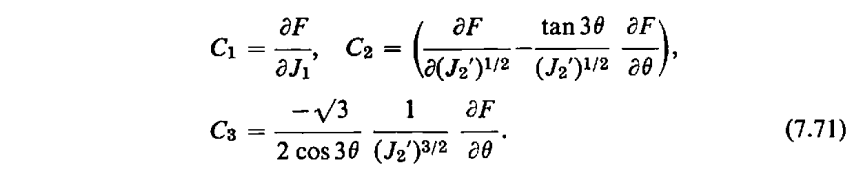
\includegraphics[width=10cm]{images/perzyna/owenhinton2}}
\end{center}

\noindent Note that we already have established (see Section~\ref{ss:recapInv}) that  
\begin{eqnarray}
\frac{\partial {\cal I}_1(\bm\sigma)}{\partial \bm\sigma} &=& {\bm 1} \\
\frac{\partial {\cal I}_2(\bm\tau)}{\partial \bm\sigma} &=& {\bm \tau} \\
\frac{\partial {\cal I}_3(\bm\tau)}{\partial \bm\sigma} 
&=& \bm\tau\cdot\bm\tau - \frac23  {\cal I}_2(\bm\tau)  {\bm 1}
\end{eqnarray}
with
\begin{eqnarray}
{\rm tr}\left[ \frac{\partial {\cal I}_1(\bm\sigma)}{\partial \bm\sigma} \right] &=& 3 \\  
{\rm tr}\left[ \frac{\partial {\cal I}_2(\bm\tau)}{\partial \bm\sigma}   \right] &=& 0 \\
{\rm tr}\left[ \frac{\partial {\cal I}_3(\bm\tau)}{\partial \bm\sigma}   \right] &=& {\rm tr}[\bm\tau\cdot\bm\tau] - 2  {\cal I}_2(\bm\tau) = 2  {\cal I}_2(\bm\tau) -2  {\cal I}_2(\bm\tau) = 0 
\end{eqnarray}

Then the generic form of the plastic potential derivative also reads
\begin{mdframed}[backgroundcolor=blue!5]
\begin{eqnarray}
\frac{\partial Q}{\partial \bm\sigma}
&=&
C_1 {\bm 1} 
+
C_2 {\bm \tau} 
+
C_3  \left( \bm\tau\cdot\bm\tau - \frac23  {\cal I}_2(\bm\tau)  {\bm 1} \right)
\end{eqnarray}
\end{mdframed}

The momentum conservation equation that we solve is 
\[
-\vec\nabla p + \vec\nabla \cdot \left[
2 \eta \dot{\bm\varepsilon}^d 
\right]+ \rho \vec g = \vec 0
\]
so we need the deviatoric strain rate tensor. 
We here assume for simplicity that there is only a visco-plastic element in the system, 
i.e. $\dot{\bm\varepsilon}=\dot{\bm\varepsilon}^{vp}$.
Then 
\begin{eqnarray}
\dot{\bm\varepsilon}^d 
&=& \dot{\bm\varepsilon}^{vp} - \frac13 {\rm tr}[ \dot{\bm\varepsilon}^{vp}] {\bm 1} \nn\\
&=& \gamma \langle \phi(F) \rangle 
\left\{
\left(C_1 \bm 1 + C_2 \bm\tau + C_3 (\bm\tau\cdot\bm\tau-\frac23 {\cal I}_2(\bm\tau)\bm 1)\right)
-\frac13
{\rm tr}
\left[C_1 \bm 1 + C_2 \bm\tau + C_3 (\bm\tau\cdot\bm\tau-\frac23 {\cal I}_2(\bm\tau)\bm 1)\right]
\bm 1
\right\} \nn\\
&=& \gamma \langle \phi(F) \rangle 
\left\{
\left(C_1 \bm 1 + C_2 \bm\tau + C_3 (\bm\tau\cdot\bm\tau-\frac23 {\cal I}_2(\bm\tau)\bm 1)\right)
-\frac13 3C_1
\bm 1
\right\} \nn\\
&=& \gamma \langle \phi(F) \rangle 
\left(C_2 \bm\tau + C_3 (\bm\tau\cdot\bm\tau-\frac23 {\cal I}_2(\bm\tau)\bm 1)\right)
\end{eqnarray}
The $C_{1,2,3}$ coefficients have been computed in 
Sections~\ref{sec:vMcriterion}, \ref{sec:trcriterion}, \ref{sec:dpcriterion} and 
\ref{sec:mccriterion}, and are summarized below: 

\begin{center}
\begin{footnotesize}
\begin{tabular}{lccc}
\hline
& $C_1$ & $C_2(\times \frac{1}{2 \sqrt{{\cal I}_2({\bm \tau})}})$ & $C_3$ \\
              \hline\hline
Tresca         &0 & $2 \cos\theta_{\rm L} ( 1 + {\color{teal}2} \tan\theta_{\rm L}  \tan 3\theta_{\rm L})$ &
$\frac{\sqrt{3}}{{\cal I}_2({\bm \tau}) } \frac{\sin\theta_{\rm L} }{\cos 3\theta_{\rm L}}$
\\ \\
von Mises      &0& {\color{teal}1}& 0 \\ \\ 
Mohr-Coulomb   & $\frac13 \sin\phi$ & 
$
\cos \theta_{\rm L} \left[
(1 +  {\color{teal}2}\tan \theta_{\rm L}   \tan 3\theta_{\rm L})
+\frac{1}{\sqrt{3}} \sin\phi
( {\color{teal}2}\tan 3\theta_{\rm L} - \tan\theta_{\rm L}) \right]$
&
$\frac{\sqrt{3}\sin\theta_{\rm L} +  \sin \phi \cos \theta_{\rm L}}
{2 {\cal I}_2({\bm \tau}) \cos 3\theta_{\rm L}}$ 
\\ \\
Drucker-Prager & $\alpha$ & 1 & 0 \\  
\hline
\end{tabular}
\end{footnotesize}
\end{center}
The differences with the table below  taken from \textcite{owhi} are highlighted in blue.
The difference in the von Mises simply comes from the definition of the 
yield value.

\begin{center}
\fbox{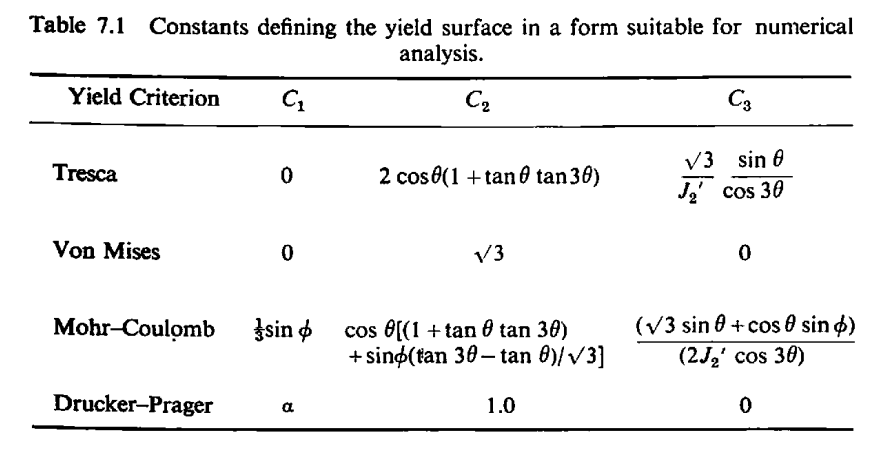
\includegraphics[width=12cm]{images/perzyna/owenhinton1}}\\
{\captionfont Taken from \textcite{owhi}.
This table supposedly presents all three $C_{1,2,3}$ coefficients 
for all four plastic potentials/yield functions (associative plasticity).
This is however not the case: the $C_2$ column is not $C_2$ but 
$\partial F/\partial\sqrt I_2$!
}
\end{center}


Also, the continuity equation for incompressible flow contains the divergence 
of the velocity field, and in this case 
\[
\vec\nabla\cdot\vec\upnu = {\rm tr}[\dot{\bm\varepsilon}^{vp}] =  \gamma \langle \phi(F) \rangle  3 C_1
\]
%If $C_3=0$, as in the vM or DP case, then we have a relationship between
%deviatoric strain rate and stress that involves a scalar. 
%If not, then a 4th order tensor is needed. This is bad news. 
%Then, vM and Tresca do not modify the continuity equation as $C_1=0$.

I find it difficult to wrap my head around this as the continuity equation 
is usually derived by other means. 
If $C_1$ is not zero, then dilation occurs, the material is not incompressible
so density should also change...  


%-------------------------------------------------------------------------------------------------
\subsubsection{von Mises plasticity following Zienkiewicz (1975)}

%In this case $F^{\text{\tiny vM}}= \sqrt{{\cal I}_2(\bm\tau)} - Y$.
%and 
%$Q^{\text{\tiny vM}}=\sqrt{{\cal I}_2(\bm\tau)}$.
What follows is borrowed from Zienkiewicz (1975) \cite{zien75}.

%Let us start by recalling the effective deviatoric stress 
%and strain rates once again:
%\begin{equation}
%\tau_{e}=\sqrt{{\cal I}_2({\bm \tau})}
%\quad\quad\quad
%\dot{\varepsilon}_{e}=\sqrt{{\cal I}_2(\dot{\bm \varepsilon}^d)}
%\end{equation}

\begin{center}
\fbox{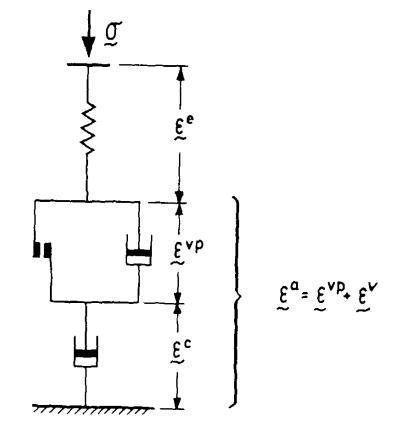
\includegraphics[width=6cm]{images/perzyna/zien75}}\\
{\captionfont Taken from \textcite{zien75}.}
\end{center}

We start from section 13.4.2 of the paper with the Perzyna formulation of the plastic strain
\footnote{from which I have removed the unnecessary/uncommon $\sqrt 3$ terms}. 
\[
\dot{\bm \varepsilon}^{vp} = \gamma \langle \phi(F) \rangle \frac{\partial Q}{\partial \bm\sigma}
\]
Associative plasticity is used, i.e. $F^{\text{\tiny vM}}=Q^{\text{\tiny vM}}$, and the von Mises yield
criterion is $F^{\text{\tiny vM}}=\sqrt{{\cal I}_2(\bm \tau)}- Y$ so
\begin{eqnarray}
\dot{\bm \varepsilon}^{vp} 
&=& \gamma \Big\langle \phi\left(\sqrt{{\cal I}_2(\bm \tau)}- Y\right)  \Big\rangle 
\frac{\partial (\sqrt{{\cal I}_2(\bm \tau)}- Y)}{\partial \bm\sigma} \nn\\
&=& \gamma \big\langle \phi\left(\sqrt{{\cal I}_2(\bm \tau)}- Y\right)  \Big\rangle 
\frac{\partial \sqrt{{\cal I}_2(\bm \tau)}}{\partial \bm\sigma} \nn\\
&=& \gamma \Big\langle \phi\left(\sqrt{{\cal I}_2(\bm \tau)}- Y\right)  \Big\rangle 
\frac{1}{2 \sqrt{{\cal I}_2(\bm \tau)}} \frac{\partial {\cal I}_2(\bm \tau)}{\partial \bm\sigma}
\end{eqnarray}
Using results of Section~\ref{ss:recapInv} for the partial derivative of the second invariant
we find\footnote{This is the same equation as Eq.~(14) of 
\textcite{zijo78}}:
\begin{eqnarray}
\dot{\bm \varepsilon}^{vp} 
&=& \gamma \Big\langle \phi\left(\sqrt{{\cal I}_2(\bm \tau)}- Y \right)  \Big\rangle 
\frac{1}{2 \sqrt{{\cal I}_2(\bm \tau)}} {\bm \tau}
\end{eqnarray}
which we can also write\footnote{There most likely is a confusion in 
the paper between $\sigma$ and $\tau$ there.}
\[
\dot{\bm \varepsilon}^{vp} =
\frac{1}{2\eta} \bm\tau
\qquad
{\rm with}
\qquad
\frac{1}{2\eta} = \gamma \Big\langle \phi(\sqrt{{\cal I}_2(\bm \tau)}- Y) \Big\rangle 
\frac{1}{2 \sqrt{{\cal I}_2(\bm \tau)}}
\]
Note that it here follows that the flow is incompressible since 
the visco-plastic strain rate tensor is proportional to the deviatoric stress tensor
so it is deviatoric itself!

%Interestingly the author then states:
%``As mentioned before this form is convenient for solving problems with
%prescribed tractions. We now seek a form of $\bm\Gamma$ which will 
%be applicable for prescribed velocity problems.'' Not sure what to make of it, though.

From the definition of the second moment invariant:
\[
{\cal I}_2(\bm\tau)
=\frac12 \bm\tau:\bm\tau 
=\frac12 (2\eta \dot{\bm \varepsilon}^{vp}):(2\eta \dot{\bm \varepsilon}^{vp})
=4 \eta^2   \frac12 \dot{\bm \varepsilon}^{vp}: \dot{\bm \varepsilon}^{vp}
=4\eta^2 {\cal I}_2(\dot{\bm \varepsilon}^{vp})
\]
from which $\eta$ can be found as a function of strain rates and 
hence $\bm\Gamma(\dot{\bm\varepsilon})$ becomes available.
Note that annoyingly the author defines the second invariant as 
$2 \dot{\bm\varepsilon}:\dot{\bm\varepsilon}$ in Eq.~(13.50) of the paper.

It follows that 
\[
\tau_e =\sqrt{{\cal I}_2(\bm\tau)}=2\eta \dot{\varepsilon}_e^{vp}
\]

Then we drop the $\langle \cdot \rangle$ as we assume to be above yield and 
we also assume a power-law form $\phi(F)=F^n$ so that 
we can solve explicitly for $\eta$:

\begin{eqnarray}
\frac{1}{2\eta} 
&=& \gamma \Big\langle \phi(\sqrt{{\cal I}_2(\bm \tau)}- Y)  \big\rangle 
\frac{1}{2 \sqrt{{\cal I}_2(\bm \tau)}} \nn\\
\frac{1}{2\eta} 
&=& \gamma \left(2\eta \sqrt{{\cal I}_2(\dot{\bm\varepsilon})}- Y\right)^n  \frac{1}{2 \; 2 \eta \sqrt{{\cal I}_2(\dot{\bm\varepsilon})}} \nn\\
\frac{1}{2\eta} 
&=& \gamma \left(2\eta \dot\varepsilon_e - Y\right)^n  \frac{1}{2 \; 2 \eta \dot\varepsilon_e } \nn\\
2 \dot\varepsilon_e
&=& \gamma (2\eta \dot\varepsilon_e - Y)^n  \nn\\
2 \dot\varepsilon_e / \gamma
&=&  (2\eta \dot\varepsilon_e - Y)^n  \nn\\
(2 \dot\varepsilon_e / \gamma)^{1/n}
&=&  2\eta \dot\varepsilon_e - Y \nn\\
\eta &=& \frac{ Y + (2 \dot\varepsilon_e / \gamma)^{1/n}}{2  \dot\varepsilon_e}
\end{eqnarray}
This form is convenient for plastic, visco-plastic and creep phenomena\footnote{Down 
to various $\sqrt{2}$ or $\sqrt{3}$ coefficients here or there, it 
is also to be found in Vilotte etal \cite{vidm82,vidm84,vimd86}}.
This can be re-written
\begin{eqnarray}
\eta 
&=& \frac{ Y + (2 \dot\varepsilon_e / \gamma)^{1/n}}{2  \dot\varepsilon_e} \nn\\
&=& \frac{ Y }{2  \dot\varepsilon_e}
+ \frac{ (2 \dot\varepsilon_e / \gamma)^{1/n}}{2  \dot\varepsilon_e} \nn\\
&=& \frac{ Y }{2  \dot\varepsilon_e}
+ \frac{ (2  / \gamma)^{1/n}}{2 }   \dot\varepsilon_e^{\frac1n-1} \nn\\
&=& \frac{ Y }{2  \dot\varepsilon_e}
+ \frac{1 }{2 } (\gamma/2)^{-1/n}  \dot\varepsilon_e^{\frac1n-1} 
\label{eq:zien75:a}
\end{eqnarray}
We often use dislocation creep/power-law rheologies and these yield an effective 
viscosity $\frac12 A^{-1/n} \dot\varepsilon_e^{\frac1n-1}$ (the temperature and/or 
pressure-dependent exponential has been omitted for simplicity - it is a power law rheology).
The equation above is then the sum of the 'plastic viscosity' and the 'viscous creep viscosity' 
-- which corresponds to a dashpot and a plastic element in parallel.
Note that the expression above is very similar to the one for Bingham or Herschel-Bulkley visco-plastic
models.

If $n=1$ then we find (as in Vilotte \etal (1982) \cite{vidm82})
\begin{eqnarray}
\eta 
&=& \frac{ Y }{2  \dot\varepsilon_e}
+ \frac{1 }{\gamma } 
\end{eqnarray}
and $\gamma$ is then the inverse of the (linear) viscosity of the dashpot.
Also if $n=1$ then $\bar\eta=\gamma^{-1}$.

For pure plasticity then $\gamma \rightarrow \infty$ and we have here simply
\[
\eta = \frac{Y}{2  \dot\varepsilon_e}
\]
As stated in Vilotte etal (1982) \cite{vidm82}: ``The plastic
flow law of Eq.~\eqref{eq:zien75:a} permits us to
represent in a single expression both the rigid-perfectly plastic flow
($\gamma\rightarrow \infty$)
and the common power creep law without plastic limit ($Y=0$)
(usually referred to as the Norton-Hoff law)\footnote{\url{https://en.wikipedia.org/wiki/Viscoplasticity}}''.
\textcite{vidm82} then explain that the fluidity $\gamma$ can depend on 
temperature $T$ in the form 
\[
\gamma = \gamma_0 \exp(-Q/RT)
\]
In conclusion we find that this formulation allows us to represent linear, power law,
perfectly plastic and visco-plastic materials.
Also, we know that the additional term $\bar\eta=\gamma^{-1}$ introduces a length scale
in the shear bands by limiting the viscosity value in said shear bands.

Remarks:
%%--------------------------------------------------------------------
%\subsection{Looking at other yield criteria \& various remarks}

%In the previous section the quantity $Y$ does not need to be a constant.
%For instance, the Drucker-Prager yield criterion can also be cast as
%$F= \sqrt{{\cal I}_2(\bm\tau)} - Y$ with $\alpha {\cal I}_1(\bm\sigma)+k$.
%Likewise the Mohr-Coulomb yield criterion of Eq.~\eqref{eq:mcF} can be written:
%\begin{equation}
%F^{\text{\tiny MC}}=
%\sqrt{  {\cal I}_2({\bm \tau})  } 
%- \frac{ c \cos \phi - \frac{1}{3} {\cal I}_1({\bm \sigma}) \sin \phi }{
%\cos \theta - \frac{1}{\sqrt{3}} \sin \theta  \sin \phi 
%}
%\end{equation}

If we use a non-associative plasticity then often $Q=\sqrt{{\cal I}_2(\bm\tau)}$.
and the formulation of the previous section remains valid. In that case 
we have $C_1=0$ and $C_3=0$ which allows to easily arrive at a relationship 
of the type $\dot{\bm\varepsilon}^{vp} = \frac{1}{2\eta} \bm\tau$ where 
$\eta$ is a scalar viscosity. 

However, if $Q$ is such that $C_3\neq 0$, then we have a problem because 
even by setting $n=1$ I do not know how to arrive at a scalar viscosity, 
and even thinking of $\eta$ as a tensor then I am stuck, see Section about 
Choi \& Petersen (2015).





\newpage
%----------------------------------------------------
\subsubsection{Dissecting Choi \& Petersen (2015)}

For implementation details, please look at \stone~39. 

The original paper \cite{chpe15} is in 2D and focuses on the MC criterion. 
The authors state that the conservation of mass equation 
should be 
\[
\frac{\partial v_x}{\partial x}
+
\frac{\partial v_y}{\partial y}
=
R=2 \sin \psi \; \dot{\varepsilon}^p
\]
where where $R$ is the dilation rate, $\Psi$ is the dilation angle and
$\dot{\varepsilon}^p$ is the square root of the second invariant of the deviatoric plastic strain rate tensor.

After multiple reads, I originally had many questions:
\begin{itemize}
\item where does this dilation rate $R$ come from ? 
\item after reading \textit{many} papers or textbooks on plasticity 
I cannot see a factor 2 in an equation anymore without re-deriving 
it from scratch with a coherent set of notations (preferably mine in fieldstone). 
\item is this relationship still valid in 3D?
\item is it the same term for Drucker-Prager ?
\end{itemize}

\vspace{1cm}

Let us first look at their Eq.~(3)  in which  
the MC yield function is given by the function $f$:
\[
f = \sigma_1 - N_\phi \sigma_3 - 2 \sqrt{N_\phi} c 
\]
where $\sigma_1$ and $\sigma_3$ are the greatest and the least principal stress, $N_\phi=(1+\sin \phi)/(1-\sin \phi)$.
This is a somewhat unusual formulation in the geodynamics community.

Let us then start with the MC yield criterion\footnote{\url{https://en.wikipedia.org/wiki/Mohr-Coulomb_theory}}
\begin{equation}
\tau_m = \sigma_m \sin \phi + c \cos \phi  \label{eq:mccrit}
\end{equation}
which means that compression is assumed to be positive (the opposite as in fieldstone) and where $\tau_m$ is the magnitude of the shear stress, 
$\sigma_m$ is the normal stress, $c$ is the intercept of the failure envelope with the $\tau$ axis, 
and $\phi$ is the slope of the failure envelope. 
The quantity $c$ is called the cohesion and the angle $\phi$ is called the angle of internal friction.
We have
\[
\sigma_m=\frac{1}{2}(\sigma_1+\sigma_3) 
\]
and 
\[
\tau_m = \frac{1}{2}(\sigma_1-\sigma_3)
\]
Inserting these into Eq.~\eqref{eq:mccrit}
\begin{equation}
 \frac{1}{2}(\sigma_1-\sigma_3) = \frac{1}{2}(\sigma_1+\sigma_3)  \sin \phi + c \cos \phi 
\end{equation}
which can be reworked as follows:
\[
\sigma_1 - \frac{1 + \sin\phi}{1-\sin\phi} \sigma_3 - 2 \frac{\cos \phi}{1-\sin\phi} c = 0
\]
The third term can further be modified as follows:
\[
\frac{\cos \phi}{1-\sin\phi}
=\frac{\sqrt{1-\sin^2 \phi}}{\sqrt{(1-\sin\phi)^2}}
=\frac{\sqrt{(1-\sin \phi)(1+\sin\phi)}}{\sqrt{(1-\sin\phi)^2}}
=\sqrt{
\frac{1+\sin\phi}{1-\sin\phi}
}
\]
Finally, we define $N_\phi$ as follows 
\[
N_\phi=\frac{1+\sin \phi}{1-\sin\phi}
\]
so that the yield condition becomes:
\[
\sigma_1 - N_\phi \sigma_3 - 2 \sqrt{N_\phi} \; c = 0
\]
which is Eq.~3 of the article by Choi \& Petersen \cite{chpe15}.

They also define the plastic potential as 
\[
g=\sigma_1 -N_\psi \sigma_3  =\tau_m - \sigma_m \sin\psi
\]

We start again from the M-C criterion (in this case $\sigma_2$ replaces $\sigma_3$):
\begin{eqnarray}
\frac{1}{2}(\sigma_1-\sigma_2) &=& - \frac{1}{2}(\sigma_1+\sigma_2)  \sin \phi + c \cos \phi  \nn\\
\end{eqnarray}
In the case of incompressible flow I have established in Section~\ref{ss:plane_strain} that 
\begin{eqnarray}
\frac{\sigma_1+\sigma_2}{2} &=& \frac{\sigma_{xx}+\sigma_{yy}}{2} = \frac12 {\cal I}_1(\bm\sigma)\\
\frac{\sigma_1-\sigma_2}{2} &=& \sqrt{ \left(\frac{\sigma_{xx}-\sigma_{yy}}{2}\right)^2 + \sigma_{xy}^2  }
=\sqrt{ {\cal I}_2(\bm\tau)  }
\end{eqnarray}
so that we now have
\[
F^{\text{\tiny MC}} 
= \frac{1}{2}{\cal I}_1(\bm\sigma) \sin\phi  + 
\sqrt{ {\cal I}_2(\bm\tau)  }
-c \cos \phi 
\]
and then the plastic potential $Q$ is given by
\[
Q^{\text{\tiny MC}}=\frac{1}{2}{\cal I}_1(\bm\sigma) \sin\psi  + \sqrt{ {\cal I}_2(\bm\tau)  }
\]
We will need $\partial Q/\partial \bm\sigma$.
By applying the chain rule we can write
\begin{eqnarray}
\frac{\partial Q}{\partial \bm\sigma} 
&=&
\frac{\partial Q}{\partial {\cal I}_1(\bm\sigma)} 
\frac{\partial {\cal I}_1(\bm\sigma)}{\partial \bm\sigma} 
+
\frac{\partial Q}{\partial {\cal I}_2(\bm\tau)} 
\frac{\partial {\cal I}_2(\bm\tau)}{\partial \bm\sigma} \nn\\
&=&
\frac{\partial Q}{\partial {\cal I}_1(\bm\sigma)} 
\frac{\partial {\cal I}_1(\bm\sigma)}{\partial \bm\sigma} 
+
\frac{\partial Q}{\partial \sqrt{{\cal I}_2(\bm\tau)}} 
\frac{\partial \sqrt{ {\cal I}_2(\bm\tau)}   }{\partial {\cal I}_2(\bm\tau)} 
\frac{\partial {\cal I}_2(\bm\tau)}{\partial \bm\sigma} \nn\\
&=&
\frac12 \sin\psi \; {\bm 1} + \frac{1}{2 \sqrt{ {\cal I}_2(\bm\tau)}} 
\bm\tau
\end{eqnarray}

Ultimately we would like to be able to write $\dot{\bm \varepsilon}^{vp} = \bm\tau /(2\eta)$
where $\eta$ is the 'viscoplastic' viscosity. However, as opposed to Zienkiewicz (1975) in the 
previous section, the term $\partial Q/\partial \bm\sigma$
is not directly/only proportional to the deviatoric stress $\bm\tau$ and we have instead:

\begin{eqnarray}
\dot{\bm \varepsilon}^{vp} 
&=& \gamma \big\langle \phi( F^{\text{\tiny MC}} )  \big\rangle 
\left(\frac12 \sin\psi \;  {\bm 1} + \frac{1}{2 \sqrt{{\cal I}_2(\bm \tau)}} {\bm \tau} \right)
\end{eqnarray}
Right away we note that the strain rate tensor above is not deviatoric, i.e. the flow
is not incompressible.
Rather conveniently, the M-C criterion in plane strain can also 
be cast $F^{\text{\tiny MC}} = \sqrt{{\cal I}_2(\bm \tau)} -Y = \tau_e - Y$ as in 
the von Mises case, albeit with 
$Y= -\frac12 {\cal I}_1(\bm\sigma) \sin\phi + c\cos\phi$.
Assuming $\phi(x)=x$ for convenience here and the argument of the brackets is positive, 
\begin{eqnarray}
\dot{\bm \varepsilon}^{vp} 
&=& \gamma \left(\sqrt{{\cal I}_2(\bm\tau)} - Y \right)
\left(\frac12 \sin\psi \;  {\bm 1} + \frac{1}{2 \sqrt{{\cal I}_2(\bm \tau)}} {\bm \tau} \right) \nn\\
&=& \gamma \left(\sqrt{{\cal I}_2(\bm\tau)} - Y \right)
\frac12 \sin\psi \;  {\bm 1} 
+  
\gamma \left(\sqrt{{\cal I}_2(\bm\tau)} - Y \right)
\frac{1}{2 \sqrt{{\cal I}_2(\bm \tau)}} {\bm \tau}  \nn\\
&=& \gamma \left(\tau_e - Y \right)
\frac12 \sin\psi \;  {\bm 1} 
+  
\gamma \left(\tau_e - Y \right)
\frac{1}{2 \tau_e} {\bm \tau}  \label{eq:evpcp15}
\end{eqnarray}
If we follow the procedure of Zienkiewicz (1975) , then the deviatoric part
of the equation above would yield a 
viscosity
\begin{eqnarray}
\eta 
&=& \frac{Y}{2  \dot\varepsilon_e^{vp}}
+ \frac{1 }{\gamma } 
\qquad \Rightarrow \qquad 
\tau_e = 2\eta \dot\varepsilon_e^{vp} = Y + \gamma^{-1} 2  \dot\varepsilon_e^{vp}
\qquad 
\Rightarrow
\qquad
\tau_e - Y = \gamma^{-1} 2  \dot\varepsilon_e^{vp}
\end{eqnarray}
If we insert this in Eq.~\eqref{eq:evpcp15}: 
\begin{eqnarray}
\dot{\bm \varepsilon}^{vp} 
&=& \gamma 
\gamma^{-1} 2  \dot\varepsilon_e^{vp}
\frac12 \sin\psi \;  {\bm 1} 
+  
\frac{1}{2\eta}
{\bm \tau}  \nn\\
&=& 
\dot\varepsilon_e^{vp}
\sin\psi \;  {\bm 1} 
+  
\frac{1}{2\eta}
{\bm \tau}  
\end{eqnarray}
Assuming that the total strain rate is the sum of the strain rates 
associated to the various deformation mechanisms, and that all
other deformation mechanisms are deviatoric, then 
\[
div (\vec\upnu)=
\dot{\varepsilon}_{xx}
+
\dot{\varepsilon}_{yy}
=
2  \dot\varepsilon_e^{vp}
\sin\psi 
\]
This 
is identical to the
dilation rate of \textcite{chpe15}!



%--------------------------------------------------------
\subsubsection{my take on this in 3D for Drucker-Prager}


I have established in Section~\ref{ss:dpcriterion} that in the general 3D case
\begin{equation}
F^{\text{\tiny DP}}= \alpha(\phi,c) {\cal I}_1({\bm \sigma}) + \sqrt{ {\cal I}_2({\bm \tau})  } + k(\phi,c) 
=\sqrt{  {\cal I}_2({\bm \tau})  } -Y 
\end{equation}
with $\alpha$ and $k$ being functions of the cohesion $c$ and angle of friction $\phi$ 
(but not from the stress). Then the plastic potential is
\begin{equation}
Q^{\text{\tiny DP}}= \alpha(\psi,c) {\cal I}_1({\bm \sigma})   +  \sqrt{  {\cal I}_2({\bm \tau})  } 
\end{equation}
where $\psi$ is the dilation angle.
We then have
\begin{eqnarray}
\frac{\partial Q}{\partial \bm\sigma} 
&=&
\frac{\partial Q}{\partial {\cal I}_1(\bm\sigma)} 
\frac{\partial {\cal I}_1(\bm\sigma)}{\partial \bm\sigma} 
+
\frac{\partial Q}{\partial \sqrt{{\cal I}_2(\bm\tau)}} 
\frac{\partial \sqrt{ {\cal I}_2(\bm\tau)}   }{\partial {\cal I}_2(\bm\tau)} 
\frac{\partial {\cal I}_2(\bm\tau)}{\partial \bm\sigma} 
=
\alpha(\psi,c) \; {\bm 1} + \frac{1}{2 \sqrt{ {\cal I}_2(\bm\tau)}} 
\bm\tau
\end{eqnarray}
Then 
\begin{eqnarray}
\dot{\bm \varepsilon}^{vp} 
&=& \gamma \left(\sqrt{{\cal I}_2(\bm\tau)} - Y \right)
\left(\alpha(\psi,c) \;  {\bm 1} + \frac{1}{2 \sqrt{{\cal I}_2(\bm \tau)}} {\bm \tau} \right) \nn\\
&=& \gamma \left(\tau_e - Y \right)
\alpha(\psi,c) \;  {\bm 1} 
+  
\gamma \left(\tau_e - Y \right)
\frac{1}{2 \tau_e} {\bm \tau}  
\end{eqnarray}
Using again $\tau_e - Y = \gamma^{-1} 2  \dot\varepsilon_e^{vp}$ as in the 2D case 
we arrive finally
\[
div (\vec\upnu)=
{\rm tr}[\dot{\bm \varepsilon}^{vp}]=
\dot{\varepsilon}_{xx}
+
\dot{\varepsilon}_{yy}
+
\dot{\varepsilon}_{zz}
=
6 \alpha(\psi,c) \dot\varepsilon_e^{vp}
\]
Since $k$ does not depend on stress, the only difference between the associative
and the non-associative case is whether $\phi=\psi$ or not.

%--------------------------------------
\subsubsection{my take on this in 3D for MC}

I have established in fieldstone that in the general 3D case
\begin{equation}
F^{\text{\tiny MC}}=\frac{1}{3} {\cal I}_1({\bm \sigma}) \sin \phi  + 
\sqrt{  {\cal I}_2({\bm \tau})  } \left( \cos \theta_{\rm L}(\bm\tau) - 
\frac{1}{\sqrt{3}} \sin \theta_{\rm L}(\bm\tau)  \sin \phi \right) - c \cos \phi
\end{equation}
Note that since $p=-{\cal I}_1(\bm\sigma)/3$ then we recover the usual '$p\sin\phi+c \cos\phi$'.

Following Eq.~(4) of the paper the plastic potential would be given by 
\[
Q^{\text{\tiny MC}} 
=\frac{1}{3} {\cal I}_1({\bm \sigma}) \sin \psi  + 
\sqrt{  {\cal I}_2({\bm \tau})  } 
\left( \cos \theta_{\rm L}(\bm\tau) -\frac{1}{\sqrt{3}} \sin \theta_{\rm L}(\bm\tau) \sin \psi \right) 
\]
The visco-plastic strain rate would then write
\[
\dot{\bm\varepsilon}^{vp} = \gamma \langle \phi(F^{\text{\tiny MC}}) \rangle 
\frac{\partial Q^{\text{\tiny MC}}}{\partial \bm\sigma}
\]
We have established that 
\begin{eqnarray}
\frac{\partial Q}{\partial \bm\sigma}
&=& 
C_1  \frac{\partial {\cal I}_1(\bm\sigma)}{\partial \bm\sigma} 
+
C_2  \frac{\partial {\cal I}_2(\bm\tau)}{\partial \bm\sigma} 
+
C_3  \frac{\partial {\cal I}_3(\bm\tau)}{\partial \bm\sigma}\nn\\
&=& C_1 {\bm 1} + C_2  {\bm \tau} + C_3 \left( \bm\tau\cdot\bm\tau -\frac23 {\cal I}_2(\bm\tau){\bm 1} \right)
\end{eqnarray}
and in the case of the Mohr-Coulomb criterion:
\begin{eqnarray}
C_1^{\text{\tiny MC}} &=& \frac13 \sin\phi  \\ 
C_2^{\text{\tiny MC}} 
&=& 
\frac{1}{2 \sqrt{ {\cal I}_2(\bm\tau)}   }   
\cos \theta_{\rm L}
\left[
(1 +  2\tan \theta_{\rm L}   \tan 3\theta_{\rm L})
+\frac{1}{\sqrt{3}} \sin\phi
( 2\tan 3\theta_{\rm L} - \tan\theta_{\rm L})
\right]
\nn\\
C_3^{\text{\tiny MC}} 
&=& 
\frac{
\sqrt{3}\sin\theta_{\rm L}
+
 \sin \phi \cos \theta_{\rm L}
}{2 {\cal I}_2({\bm \tau}) \cos 3\theta_{\rm L}}
\end{eqnarray}



\[
\dot{\bm\varepsilon}^{vp} = \gamma \langle \phi(F) \rangle 
\left(
C_1 {\bm 1} + C_2  {\bm \tau} + C_3 \left( \bm\tau\cdot\bm\tau -\frac23 {\cal I}_2(\bm\tau){\bm 1} \right)
\right)
\]
Assuming brackets ok, and $\phi(x)=x^n$:
\[
\dot{\bm\varepsilon}^{vp} = \gamma (\sqrt{{\cal I}_2(\bm\tau)} - Y)^n 
\left(
C_1 {\bm 1} + C_2  {\bm \tau} + C_3 \left( \bm\tau\cdot\bm\tau -\frac23 {\cal I}_2(\bm\tau){\bm 1} \right)
\right)
\]
Taking the deviatoric part of this:
\[
\dot{\bm\varepsilon}^{vp,d} 
= \gamma (\sqrt{{\cal I}_2(\bm\tau)} - Y)^n 
\left(
 C_2  {\bm \tau} + C_3 \left( \bm\tau\cdot\bm\tau -\frac23 {\cal I}_2(\bm\tau){\bm 1} \right)
\right)
\]
so I cannot find a \underline{scalar} $\eta$ such that 
\[
\dot{\bm\varepsilon}^{vp,d} 
=\frac{1}{2\eta} {\bm \tau}
\]
I am STUCK here?!


%-------------------------------------
\subsubsection{Revisiting Lemiale et al (2008) and Spiegelman et al (2016) }
The authors postulate that the total strain rate is the sum of 
the viscous deformation and plastic deformation:
\[
\dot{\bm \varepsilon} = \dot{\bm \varepsilon}^v + \dot{\bm \varepsilon}^p
\]
Then 
\begin{equation}
\bm \sigma = -p \bm 1 + 2\eta (\dot{\bm \varepsilon} -\dot{\bm \varepsilon}^p)
\label{eq:abcd}
\end{equation}
Immediately we see that they implicitely assume that the flow is incompressible.
Upon yielding a flow rule is needed to specify the plastic 
behaviour. The plastic strain rate is written as
\begin{equation}
\label{eq:lemm08:epsp}
\dot{\bm \varepsilon}^p = \dot\lambda \frac{\partial Q}{\partial \bm\sigma}
\end{equation}
where $\dot\lambda$ is a scalar plastic flow rate and $Q$ is the so-called plastic potential. 
Note that in \textcite{hesd02} the authors define $\dot{\lambda}=\langle \phi(x) \rangle/\eta$
so that the equation above is the Perzyna model. 
A classical choice for $Q$, in conjunction with the incompressibility constraint, is:
\[
Q = \sqrt{ {\cal I}_2(\bm\tau)}
\]
We notice that Eq.~\ref{eq:lemm08:epsp} is different (although obviously not unrelated) 
than the Perzyna approach above, although
in the end they arrive at a similar expression as we did before for the von Mises case.


If we consider only the deviatoric part of the stress tensor in Eq.~\eqref{eq:abcd}, we thus obtain\footnote{do they assume varepsilon deviatoric too?}
\begin{equation}
\bm \tau = 2 \eta (\dot{\bm \varepsilon} -\dot{\bm \varepsilon}^p)
= 2 \eta \left(\dot{\bm \varepsilon} - \dot\lambda \frac{\partial Q}{\partial \bm\sigma} \right)
= 2 \eta \left(\dot{\bm \varepsilon} - \dot\lambda \frac{1}{2 \sqrt{ {\cal I}_2(\bm\tau)}}  \frac{\partial {\cal I}_2(\bm\tau)}{\partial \bm\sigma} \right)
= 
2 \eta \left(\dot{\bm \varepsilon} - \dot\lambda \frac{1}{2 \sqrt{ {\cal I}_2(\bm\tau)}} \bm\tau \right) \label{eq:bcde}
\end{equation}
This equation can be written as
\[
\left( 1 + \dot\lambda \frac{\eta }{ \sqrt{ {\cal I}_2(\bm\tau)}} \right) \bm\tau
= 2 \eta \dot{\bm \varepsilon}
\]
One can then take the square root of the second invariant of this equation:
\[
\left( 1 + \dot\lambda \frac{\eta }{ \sqrt{ {\cal I}_2(\bm\tau)}} \right) 
\sqrt{{\cal I}_2(\bm\tau) }= 2 \eta \sqrt{{\cal I}_2(\dot{\bm \varepsilon})}
\]
Then 
\[
\left( 1 + \dot\lambda \frac{\eta }{ \tau_e} \right) 
\tau_e = 2 \eta \dot{\bm \varepsilon}_e
\]
so that 
\[
\dot\lambda 
= \frac{2 \eta \dot{\bm \varepsilon}_e - \tau_e}{\eta}
= 2 \dot{\bm \varepsilon}_e - \frac{\tau_e}{\eta}
\]
Finally we can insert this expression of $\dot\lambda$ in Eq.~\eqref{eq:bcde}
\begin{eqnarray}
\bm \tau 
&=&2 \eta \left(\dot{\bm \varepsilon} - \dot\lambda \frac{1}{2 \sqrt{ {\cal I}_2(\bm\tau)}} \bm\tau \right)  \\
&=& 2 \eta \left(\dot{\bm \varepsilon} -    
(2 \dot{ \varepsilon}_e - \frac{\tau_e}{\eta})
\frac{1}{2 \sqrt{ {\cal I}_2(\bm\tau)}} \bm\tau \right)  \\
&=& 2 \eta \left(\dot{\bm \varepsilon} -  
(2 \dot{ \varepsilon}_e - \frac{\tau_e}{\eta})   \frac{1}{2 \tau_e} \bm\tau \right) \\
&=& 2 \eta \dot{\bm \varepsilon} -  
2\eta \dot{\varepsilon}_e \frac{1}{ \tau_e} \bm\tau 
+ \eta \frac{\tau_e}{\eta}   \frac{1}{ \tau_e} \bm\tau \\
&=& 2 \eta \dot{\bm \varepsilon} -  
2\eta \dot{\varepsilon}_e \frac{1}{ \tau_e} \bm\tau +  \bm\tau \\
\end{eqnarray}
The term $\bm\tau$ is present on both sides of the equal sign so it cancels out
and we are left with:
\[
\bm 0 = 2 \eta \dot{\bm \varepsilon} -  
2\eta \dot{\varepsilon}_e \frac{1}{ \tau_e} \bm\tau 
\]
or,
\[
\bm\tau = \frac{\tau_e}{\dot{\varepsilon}_e}  \dot{\bm \varepsilon}
\]
On yield we have $\tau_e=Y(c,\phi)$ so in the end:
\[
{\bm\tau} = 2 \underbrace{
\frac12 \frac{Y(c,\phi)}{ \dot{\varepsilon}_e} 
}_{\eta_p}  \dot{\bm \varepsilon}
\]
That last step is poorly documented in the paper!
This is a cumbersome exercise and it relies heavily on the choice of $Q=\tau_e$.


\begin{remark}
Lemiale \etal (2008) define $\overline{\tau}=\sqrt{\tau_{ij}\tau_{ij}/2}$
but define $\dot{\gamma}=\sqrt{2 D_{ij}D_{ij}}$!
\end{remark}

Let us now turn to \textcite{spmw16} (2016).
In Section~2.1.1 of this paper the authors follow the same path as above. 
They assume $Q=\tau_e$ but justify their choice by stating that ``The use of incompressible materials mandates that we use a plastic potential g which is not a function of the pressure $p$''

This is indeed very important in the context of our incompressible calculations in geodynamics. 

They define the yield surface, $F(\bm\sigma)$ which is a scalar function defining the failure (yield) state of a material. Yield surfaces are
assumed to be of the following form 
\[
F(\bm\sigma) =\tau_e - Y(\bm\sigma)
\]
where $Y$ is the yield criterion.
The authors state that ``it is common practice in geodynamics to define the
plastic multiplier $\dot\lambda$ which exactly satisfies $F=0$, 
or equivalently $\tau_e=Y$ \cite{lemm08}''.
We see that it is then the same as the Lemiale \etal paper.





